\section{Storing the Curve History\label{arr_sec:arr_with_hist}}
%==================================

As stated at the beginning of this chapter (Section~\ref{arr_sec:intro}), 
when one constructs an arrangement induced by a set $\calC$ of arbitrary 
planar curves, she or he constructs a collection $\calC''$ of $x$-monotone 
subcurves of $\calC$ that are pairwise disjoint in their interior, and these 
subcurves are associated with the arrangement edges (more precisely, with the 
\dcel\ halfedges). Doing so, the connection between the originating input 
curves and the arrangement edges is lost. This loss might be acceptable for 
some applications. However, in many practical cases it is important to 
determine the input curves that give rise to the final subcurves.

The \ccc{Arrangement_with_history_2<Traits,Dcel>} class-template extends
the \ccc{Arrangement_2} class by keeping an additional container of input
curves representing $\calC$, and by maintaining a cross-mapping between these
curves and the arrangement edges they induce. The traits class that is
used for instantiating the template should be a model of the
\ccc{ArrangementTraits_2} concept (see Section~\ref{arr_sssec:insert_gen}).
That is, it should define the \ccc{Curve_2} type (and not just the
\ccc{X_monotone_curve_2} type). The \ccc{Dcel} parameter should model the 
\ccc{ArrangementDcel} concept. Users can use the default \dcel\ class or 
an extended \dcel\ class according to their needs.

\subsection{Traversing an Arrangement with History\label{arr_ssec:arrwh_traverse}}
%--------------------------------------------------

The \ccc{Arrangement_with_history_2} class extends the \ccc{Arrangement_2}
class, thus all the iterator and circulator types that are defined by the
arrangement class are also available in \ccc{Arrangement_with_history_2}.
The reader is referred to Section~\ref{arr_ssec:traverse} for a comprehensive
review of these functions.

As mentioned above, the \ccc{Arrangement_with_history_2} class maintains
a container of input curves, which can be accessed using curve handles.
The member function \ccc{number_of_curves()} returns the number of input 
curves stored in the container, while \ccc{curves_begin()} and 
\ccc{curves_end()} return \ccc{Arrangement_with_history_2::Curve_iterator}
objects that define the  valid range of curves that induce the arrangement.
The value type of this iterator is \ccc{Curve_2}. Moreover, the curve-iterator
type is equivalent to  \ccc{Arrangement_with_history_2::Curve_handle}, which
is used for accessing the stored curves. Conveniently, the corresponding
constant-iterator and constant-handle types are also defined.

As mentioned in the previous paragraph, a \ccc{Curve_handle} object \ccc{ch} 
serves as a pointer to a curve stored in an arrangement-with-history instance 
\ccc{arr}. Using this handle, it is possible to obtain the number of 
arrangement edges this curve induces by calling 
\ccc{arr.number_of_induced_edges(ch)}. The functions 
\ccc{arr.induced_edges_begin(ch)} and
\ccc{arr.induced_edges_end(ch)} return iterators of type
\ccc{Arrangement_with_history_2::Induced_edges_iterator} that define the
valid range of edges induced by \ccc{ch}. The value type of these iterators
is \ccc{Halfedge_handle}. It is thus possible to traverse all arrangement
edges induced by an input curve.

It is also important to be able to perform the inverse mapping. Given an
arrangement edge, we would like to be able to determine which input curve
induces it. In case the edge represents an overlap of several curves, we
should be able to trace all input curves that overlap over this edge.
The \ccc{Arrangement_with_history_2} class is extended by several member
functions that enable such an inverse mapping. Given a halfedge handle \ccc{e}
in an arrangement with history \ccc{arr}, then 
\ccc{arr.number_of_originating_curves(e)} returns the number of curves that
induce the edge (which should be 1 in non-degenerate cases, and 2 or more
in case of overlaps), while \ccc{arr.originating_curves_begin(e)} and 
\ccc{arr.originating_curves_end(e)} return 
\ccc{Arrangement_with_history_2::Originating_curve_iterator} objects that
define the range of curves that induce \ccc{e}. The value type of these
iterator is \ccc{Curve_2}.

It is possible to overlay two \ccc{Arrangement_with_history_2} instances 
instantiated by the same traits class. In this case, the resulting 
arrangement will store a consolidated container of input curves, and 
automatically preserve the cross-mapping between the arrangement edges 
and the consolidated curve set. Users can employ an overlay-traits class
to maintain any type of auxiliary data stored with the \dcel\ features
(see Section~\ref{arr_sec:overlay}).

\subsection{Modifying an Arrangement with History\label{arr_ssec:modif_traverse}}
%-------------------------------------------------

As the \ccc{Arrangement_with_history_2} class extends the \ccc{Arrangement_2}
class, it inherits the fundamental modification operations, such as 
\ccc{assign()} and \ccc{clear()}, from it. The vertex-manipulation functions
are also inherited and supported (see Sections~\ref{arr_sssec:mf_iso_verts}
and~\ref{arr_sssec:insert_point} for the details). However, there are some 
fundamental differences between the interfaces of the two classes, which we
highlight in this subsection.

The most significant difference between the arrangement-with-history class
and the basic arrangement class is the way they handle their input curves.
\ccc{Arrangement_with_history_2} always stores the \ccc{Curve_2} objects
that induce it, thus it is impossible to insert $x$-monotone curves into
an arrangement with history. The free \ccc{insert_non_intersecting_curve()}
and \ccc{insert()} that receives $x$-monotone curve (as well as
their aggregated versions) are therefore not available for
arrangement-with-history instances and only the free
\ccc{insert()} and \ccc{insert()} functions that receive
\ccc{Curve_2} (the incremental insertion function and the aggregated
insertion function) are supported --- see also
Section~\ref{arr_sssec:insert_gen}. Notice however that while the
incremental insertion function \ccc{insert(arr,c)} for an
\ccc{Arrangement_2} object \ccc{arr} does not have a return value, the
corresponding arrangement-with-history function returns a
\ccc{Curve_handle} to the inserted curve. 

As we are able to keep track of all edges induced by an input curve, we also
provide a free function that removes a curve from an arrangement. By calling
\ccc{remove(arr,ch)}, where \ccc{ch} is a valid curve handle, the given curve
is deleted from the curve container, and all edges induced solely by
this curve (i.e., excluding overlapping edges) are removed from the 
arrangement. The function returns the number of edges that have been removed.

In some cases, users may need to operate directly on the arrangement edges.
We first mention that the specialized insertion functions (see 
Section~\ref{arr_sssec:mf_insert_cv}) are not supported, as they accept
$x$-monotone curves. Insertion can only be performed via the free 
insertion-functions. The other edge-manipulation functions 
(see Section~\ref{arr_sssec:mf_halfedges}) are however available, but have 
a different interface that does not use $x$-monotone curves:
\begin{itemize}
\item Invoking \ccc{split_edge(e,p)} splits the edge \ccc{e} at a given point
\ccc{p} that lies in its interior.
\item Invoking \ccc{merge_edge(e1,e2)} merges the two given edges. There is
a precondition that \ccc{e1} and \ccc{e2} shared a common end-vertex of degree
2, and that the $x$-monotone subcurves associated with these edges are
mergeable.
\item It is possible to remove an edge by simply invoking
\ccc{remove_edge(e)}.
\end{itemize}
In all cases, the maintenance of cross-pointers for the appropriate input
curves will be done automatically.

It should be noted that it is possible to attach observers to an 
arrangement-with-history instance in order to get detailed notifications of
the changes the arrangements undergoes (see Section~\ref{arr_sec:notif} for
the details).

\subsection{Examples\label{arr_ssec:arr_hist_ex}}
%---------------------------

\begin{figure}[t]
\begin{ccTexOnly}
  \begin{center}
  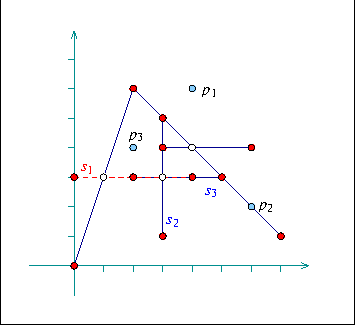
\includegraphics{Arrangement_on_surface_2/fig/ex_24}
  \end{center}
\end{ccTexOnly}
\begin{ccHtmlOnly}
  <p><center>
  <img src="./fig/ex_24.gif" border=0 alt="Example 24">
  </center>
\end{ccHtmlOnly}
\caption{An arrangement with history as constructed in
\ccc{curve_history.cpp}. 
Note that $s_1$ and $s_3$ overlap over two edges. The point-location query
points are drawn as lightly shaded dots.\label{arr_fig:ex_24}}
\end{figure}

In the following example we construct a simple arrangement of six line
segments, as depicted in Figure~\ref{arr_fig:ex_24}, while maintaining 
the curve history. The example demonstrates the usage of the special
traversal functions. It also shows how to issue point-location queries
on the resulting arrangement, using the auxiliary function 
\ccc{locate_point()} defined in the header file 
\ccc{point_location_utils.h}; see also Section~\ref{arr_ssec:pl}.

\ccIncludeExampleCode{Arrangement_on_surface_2/curve_history.cpp}

\begin{figure}[t]
\begin{ccTexOnly}
  \begin{center}
  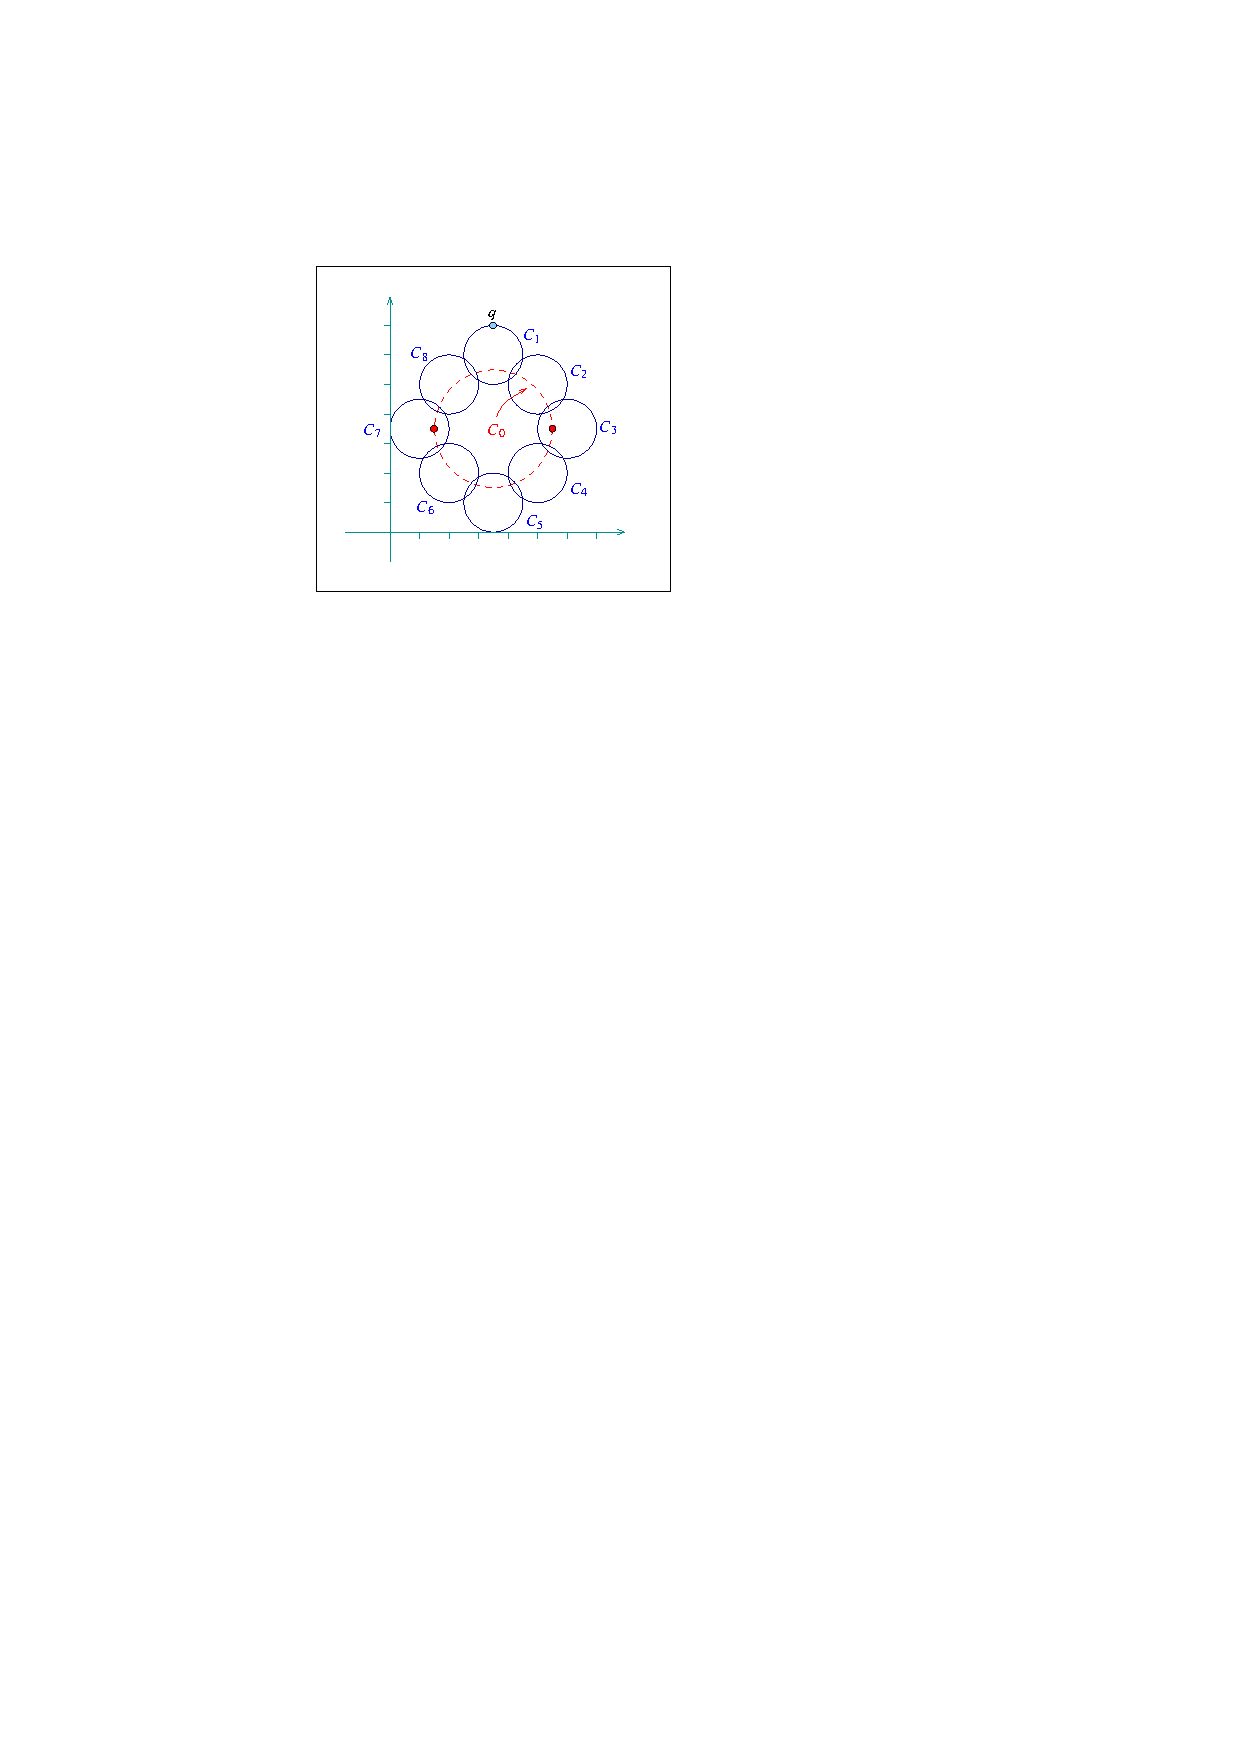
\includegraphics{Arrangement_on_surface_2/fig/ex_25}
  \end{center}
\end{ccTexOnly}
\begin{ccHtmlOnly}
  <p><center>
  <img src="./fig/ex_25.gif" border=0 alt="Example 25">
  </center>
\end{ccHtmlOnly}
\caption{An arrangement with history of nine circle as constructed in 
\ccc{edge_manipulation_curve_history.cpp}. Note the vertical tangency points
of $C_0$, marked as dark dots, which subdivide this circle into an upper half
and a lower half, each consists of 9 edges. The large circle $C_0$ is
eventually removed from the arrangement, with all 18 edges it
induces.\label{arr_fig:ex_25}}
\end{figure}

The following example demonstrates the usage of the free \ccc{remove()}
function. We construct an arrangement of nine circles, while keeping a handle
to each inserted circle. We then remove the large circle $C_0$, which induces
$18$ edges, as depicted in Figure~\ref{arr_fig:ex_25}. The example also shows
how to use the \ccc{split_edge()} and \ccc{merge_edge()} functions when
operating on an arrangement-with-history instance:

\ccIncludeExampleCode{Arrangement_on_surface_2/edge_manipulation_curve_history.cpp}
